\documentclass[border=10pt]{standalone}
\usepackage{tikz}
\usetikzlibrary{arrows,positioning,shapes.geometric}
\begin{document}
\









\tikzset{every picture/.style={line width=0.75pt}} %set default line width to 0.75pt        

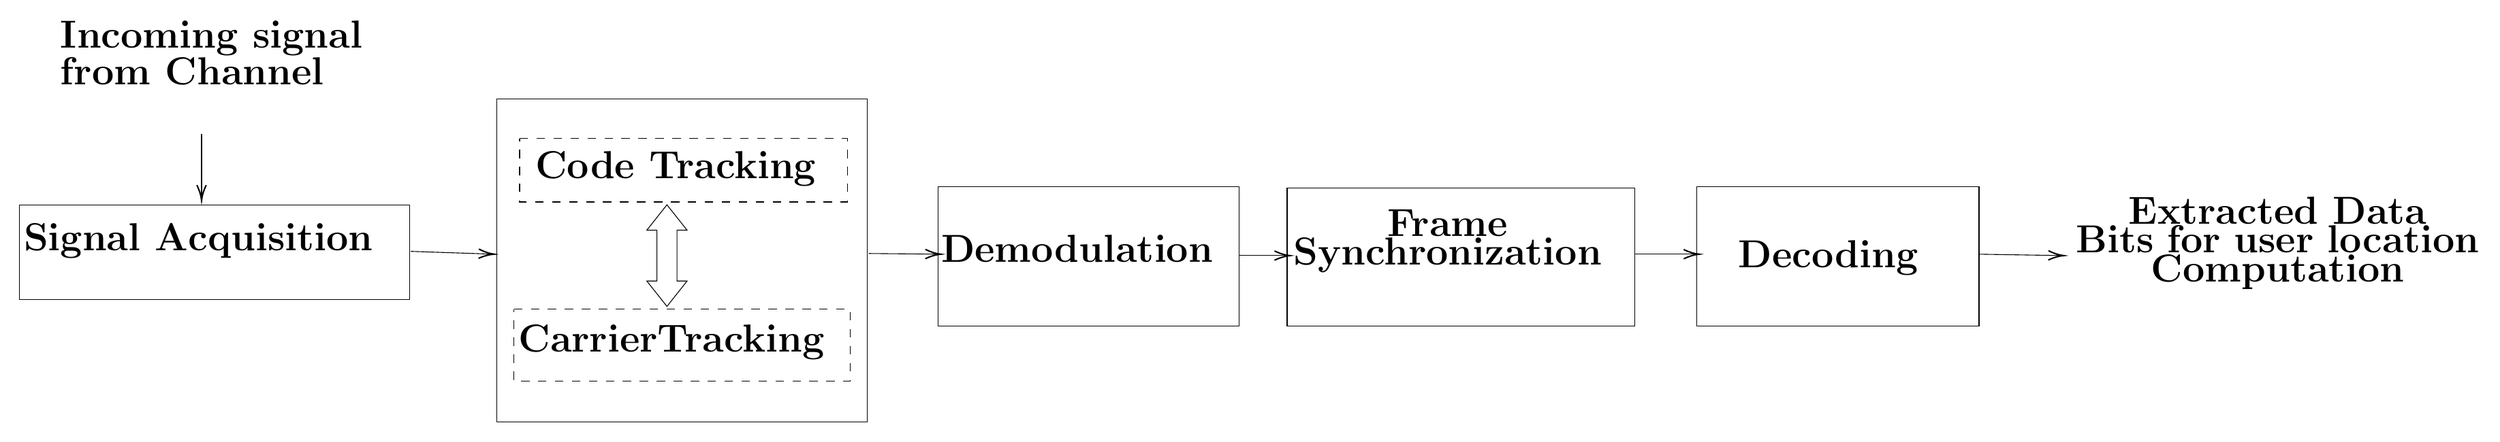
\begin{tikzpicture}[x=0.75pt,y=0.75pt,yscale=-1,xscale=1]
%uncomment if require: \path (0,421); %set diagram left start at 0, and has height of 421

%Shape: Rectangle [id:dp3971746291758471] 
\draw  [dash pattern={on 4.5pt off 4.5pt}] (363,137) -- (595,137) -- (595,182) -- (363,182) -- cycle ;
%Shape: Rectangle [id:dp25845085129393275] 
\draw   (9,184) -- (285,184) -- (285,251) -- (9,251) -- cycle ;
%Shape: Rectangle [id:dp4338649750832799] 
\draw  [dash pattern={on 4.5pt off 4.5pt}] (359,258) -- (597,258) -- (597,309) -- (359,309) -- cycle ;
%Straight Lines [id:da025296917723176437] 
\draw    (138,134) -- (138,179) ;
\draw [shift={(138,181)}, rotate = 270] [color={rgb, 255:red, 0; green, 0; blue, 0 }  ][line width=0.75]    (10.93,-3.29) .. controls (6.95,-1.4) and (3.31,-0.3) .. (0,0) .. controls (3.31,0.3) and (6.95,1.4) .. (10.93,3.29)   ;
%Shape: Rectangle [id:dp16992156871850217] 
\draw   (347,109) -- (609,109) -- (609,338) -- (347,338) -- cycle ;
%Straight Lines [id:da034679195397693485] 
\draw    (286,217) -- (343,218.93) ;
\draw [shift={(345,219)}, rotate = 181.94] [color={rgb, 255:red, 0; green, 0; blue, 0 }  ][line width=0.75]    (10.93,-3.29) .. controls (6.95,-1.4) and (3.31,-0.3) .. (0,0) .. controls (3.31,0.3) and (6.95,1.4) .. (10.93,3.29)   ;
%Up Down Arrow [id:dp0963447637089958] 
\draw   (453,202) -- (467.25,184) -- (481.5,202) -- (474.38,202) -- (474.38,238) -- (481.5,238) -- (467.25,256) -- (453,238) -- (460.13,238) -- (460.13,202) -- cycle ;
%Straight Lines [id:da4490352243030665] 
\draw    (1395,219) -- (1453.5,219.97) ;
\draw [shift={(1455.5,220)}, rotate = 180.95] [color={rgb, 255:red, 0; green, 0; blue, 0 }  ][line width=0.75]    (10.93,-3.29) .. controls (6.95,-1.4) and (3.31,-0.3) .. (0,0) .. controls (3.31,0.3) and (6.95,1.4) .. (10.93,3.29)   ;
%Shape: Rectangle [id:dp8453662584022844] 
\draw   (1196,171) -- (1395.5,171) -- (1395.5,270) -- (1196,270) -- cycle ;
%Straight Lines [id:da8952050873529491] 
\draw    (610,218.5) -- (659,218.98) ;
\draw [shift={(661,219)}, rotate = 180.56] [color={rgb, 255:red, 0; green, 0; blue, 0 }  ][line width=0.75]    (10.93,-3.29) .. controls (6.95,-1.4) and (3.31,-0.3) .. (0,0) .. controls (3.31,0.3) and (6.95,1.4) .. (10.93,3.29)   ;
%Shape: Rectangle [id:dp25594644752156004] 
\draw   (659,171) -- (872,171) -- (872,270) -- (659,270) -- cycle ;
%Shape: Rectangle [id:dp8421655608501161] 
\draw   (906,172) -- (1152,172) -- (1152,270) -- (906,270) -- cycle ;
%Straight Lines [id:da35720729664785655] 
\draw    (872,220) -- (906,220) ;
\draw [shift={(908,220)}, rotate = 180] [color={rgb, 255:red, 0; green, 0; blue, 0 }  ][line width=0.75]    (10.93,-3.29) .. controls (6.95,-1.4) and (3.31,-0.3) .. (0,0) .. controls (3.31,0.3) and (6.95,1.4) .. (10.93,3.29)   ;
%Straight Lines [id:da16424451208563873] 
\draw    (1152,219) -- (1195.5,219) ;
\draw [shift={(1197.5,219)}, rotate = 180] [color={rgb, 255:red, 0; green, 0; blue, 0 }  ][line width=0.75]    (10.93,-3.29) .. controls (6.95,-1.4) and (3.31,-0.3) .. (0,0) .. controls (3.31,0.3) and (6.95,1.4) .. (10.93,3.29)   ;

% Text Node
\draw (11,196) node [anchor=north west][inner sep=0.75pt]   [align=left] {{\huge \textbf{Signal Acquisition}}};
% Text Node
\draw (373,145) node [anchor=north west][inner sep=0.75pt]   [align=left] {{\huge \textbf{Code Tracking}}};
% Text Node
\draw (361,268) node [anchor=north west][inner sep=0.75pt]   [align=left] {\textbf{{\huge Carrier}{\Large  }{\huge Tracking}}};
% Text Node
\draw (907,186) node [anchor=north west][inner sep=0.75pt]   [align=left] {\begin{minipage}[lt]{166.94pt}\setlength\topsep{0pt}
\begin{center}
{\huge \textbf{Frame }}\\{\huge \textbf{Synchronization}}
\end{center}

\end{minipage}};
% Text Node
\draw (660,204) node [anchor=north west][inner sep=0.75pt]   [align=left] {{\huge \textbf{Demodulation}} };
% Text Node
\draw (1224,208) node [anchor=north west][inner sep=0.75pt]   [align=left] {{\huge \textbf{Decoding}}};
% Text Node
\draw (1463,177) node [anchor=north west][inner sep=0.75pt]   [align=left] {\begin{minipage}[lt]{213.89pt}\setlength\topsep{0pt}
\begin{center}
{\huge \textbf{Extracted Data }}\\{\huge \textbf{Bits for user location}}\\{\huge \textbf{Computation }}
\end{center}

\end{minipage}};
% Text Node
\draw (37,52.5) node [anchor=north west][inner sep=0.75pt]   [align=left] {{\huge \textbf{Incoming signal }}\\{\huge \textbf{from Channel}}};


\end{tikzpicture}


   
\end{document}


